\documentclass[aspectratio=169,10pt]{beamer}
\usetheme[progressbar=frametitle,numbering=fraction]{metropolis}
\usepackage[utf8]{inputenc}
\usepackage[T1]{fontenc}
\usepackage{lmodern}
\usepackage[spanish,es-noshorthands,es-tabla]{babel}
\usepackage{booktabs}
\usepackage{tikz}
\usetikzlibrary{positioning,arrows.meta,calc}

\definecolor{guinda}{HTML}{7A1F2B}
\definecolor{acento}{HTML}{C8102E}
\definecolor{okv}{HTML}{2E7D4F}
\definecolor{medv}{HTML}{A46A00}
\definecolor{altv}{HTML}{C2410C}
\setbeamercolor{frametitle}{bg=guinda}
\setbeamercolor{progress bar}{fg=acento}
\setbeamercolor{alerted text}{fg=acento}

\newcommand{\TablaCorpus}{LPDP & Perú & 17 & 64 \\
RLPDP & Perú & 60 & 175 \\
RGPD & Unión Europea & 87 & 455 \\
EDPB-07/2020 & Unión Europea & 57 & 237 \\
CCT-2021/915 & Unión Europea & -- & 47 \\}
% Generado por eval/evaluar.py — no editar a mano
\newcommand{\NumFragmentos}{978}
\newcommand{\NumClausulas}{13}
\newcommand{\HitGen}{1{,}000}
\newcommand{\MrrGen}{0{,}772}
\newcommand{\PGen}{0{,}654}
\newcommand{\PeruGen}{0{,}154}
\newcommand{\HitMix}{0{,}923}
\newcommand{\MrrMix}{0{,}733}
\newcommand{\PMix}{0{,}538}
\newcommand{\PeruMix}{0{,}692}
\newcommand{\LatRec}{64}
\newcommand{\Corridas}{3}
\newcommand{\Exactitud}{87{,}2\,\%}
\newcommand{\ExactitudBin}{92{,}3\,\%}
\newcommand{\Estabilidad}{89{,}7\,\%}
\newcommand{\MaePct}{5{,}6}
\newcommand{\LatRev}{32{,}0}
\newcommand{\CitasVer}{98{,}9\,\%}
\newcommand{\TablaContratos}{Completo (NubeSegura) & 100{,}0 & 96{,}8 & 93{,}5--98{,}4 & 89{,}7\,\% \\
Intermedio (PagoFácil) & 59{,}7 & 54{,}8 & 54{,}8--54{,}8 & 92{,}3\,\% \\
Deficiente (MailRápido) & 17{,}7 & 26{,}3 & 21{,}0--30{,}6 & 79{,}5\,\% \\}
\newcommand{\ConfCumpleCumple}{47}
\newcommand{\ConfCumpleParcial}{7}
\newcommand{\ConfCumpleFalta}{0}
\newcommand{\ConfParcialCumple}{2}
\newcommand{\ConfParcialParcial}{18}
\newcommand{\ConfParcialFalta}{1}
\newcommand{\ConfFaltaCumple}{0}
\newcommand{\ConfFaltaParcial}{5}
\newcommand{\ConfFaltaFalta}{37}
\newcommand{\ExactitudVi}{84{,}6\,\%}
\newcommand{\ExactitudBinVi}{87{,}2\,\%}
\newcommand{\EstabilidadVi}{76{,}9\,\%}
\newcommand{\MaePctVi}{8{,}1}
\newcommand{\CitasVerVi}{90{,}8\,\%}


\title{Agente de Terceros (DPAs)}
\subtitle{PIMS multiagente basado en ISO/IEC 27701:2025 --- revisión asistida de contratos de encargo}
\author{Dylan Antonio Zúñiga Huarca \and Jeferson Joao Basurco Casani \and Adrian Issac Mamani Quispe}
\institute{Auditoría de Sistemas · Escuela Profesional de Ingeniería de Sistemas · UNSA}
\date{\today}

\begin{document}
\maketitle

\begin{frame}{Problema}
\begin{columns}[T]
\column{.55\textwidth}
\begin{itemize}
  \item Hosting, planillas, pagos, \emph{mailing}: los \alert{encargados} tratan datos por cuenta nuestra.
  \item La responsabilidad \alert{sigue siendo nuestra}; la principal garantía es el \alert{contrato de encargo (DPA)}.
  \item Revisar cada DPA frente a la LPDP, el RLPDP y el RGPD art. 28 es una tarea \alert{manual, lenta y propensa a omisiones}.
  \item Hay que vigilar además vencimientos, subencargados e incidentes.
\end{itemize}
\column{.42\textwidth}
\begin{block}{Contexto peruano}
\small \textbf{LPDP art. 30}: el encargado no puede usar los datos con otro fin y debe suprimirlos al terminar.\\[2pt]
\textbf{RLPDP arts. 28-33}: tercerización, encargo y subcontratación.\\[2pt]
\textbf{RLPDP art. 36}: el encargado informa de inmediato los incidentes.
\end{block}
\end{columns}
\end{frame}

\begin{frame}{El PIMS multiagente y nuestro agente}
\begin{center}
\begin{tikzpicture}[font=\small,
  ag/.style={draw,rounded corners,minimum width=25mm,minimum height=10mm,align=center},
  on/.style={ag,fill=acento!15,draw=acento,very thick}]
\node[draw,rounded corners,fill=guinda!10,minimum width=110mm,minimum height=8mm] (o) at (0,2.2) {Orquestador + panel HITL};
\node[draw,dashed,minimum width=110mm,minimum height=5mm,font=\scriptsize] (bus) at (0,1.35) {Bus MCP (JSON-RPC)};
\foreach \t/\x/\y in {Inventario de datos/-4.2/0.2, Riesgos (DPIA)/-1.4/0.2, Controles y SoA/1.4/0.2, Evidencia y auditoría/4.2/0.2,
                      Derechos (DSAR)/-4.2/-1.1, Incidentes y brechas/-1.4/-1.1, Formación/4.2/-1.1}
  \node[ag] at (\x,\y) {\t};
\node[on] at (1.4,-1.1) {\textbf{Terceros (DPAs)}};
\end{tikzpicture}
\end{center}
\small Controles ISO/IEC 27701:2025: \alert{A.1.2.7} contratos con encargados · \alert{A.2.5.7} divulgación de subcontratistas · \alert{A.2.5.8} contratación de subencargados.
\end{frame}

\begin{frame}{Encargado: Perú frente a la Unión Europea}
\small
\begin{tabular}{@{}p{.2\textwidth}p{.38\textwidth}p{.36\textwidth}@{}}
\toprule
 & \textbf{Perú (LPDP + RLPDP)} & \textbf{UE (RGPD)} \\
\midrule
Fin limitado & LPDP 30; RLPDP 29.2, 33 & Art. 28.3.a, 28.10 \\
Subencargados & Autorización previa; el encargado prueba (RLPDP 32) & Autorización + aviso de cambios (28.2, 28.4) \\
Incidentes & Informe \alert{inmediato} (RLPDP 36) & Sin dilación indebida (33.2) \\
Fin del servicio & Supresión \alert{evidenciada}; hasta 2 años (RLPDP 30.4, 31.2) & Supresión o devolución (28.3.g) \\
Transferencias & LPDP 15; RLPDP 12-14 & Arts. 44-46 \\
\bottomrule
\end{tabular}
\vspace{4pt}

\footnotesize Referencias de buenas prácticas: Directrices 07/2020 del CEPD y cláusulas tipo de la Decisión (UE) 2021/915.
\end{frame}

\begin{frame}{Qué hace el agente}
\begin{columns}[T]
\column{.5\textwidth}
\begin{enumerate}
  \item \alert{Registro} de encargados: datos que tratan, sistemas, país y certificaciones.
  \item \alert{Revisión de DPAs} contra 13 cláusulas mínimas, con citas.
  \item \alert{Riesgo} del proveedor: probabilidad × impacto.
  \item \alert{Alertas} de vencimiento de los DPAs (60 días).
  \item \alert{Subencargados}: todo cambio requiere aprobación.
  \item \alert{Brechas}: ¿qué encargados tratan los datos afectados?
\end{enumerate}
\column{.46\textwidth}
\begin{block}{Herramientas MCP}
\texttt{list\_processors}\\
\texttt{check\_dpa\_status}\\
\texttt{evaluate\_vendor}\\
\texttt{processors\_in\_breach}
\end{block}
\begin{alertblock}{Puerta HITL}
Ningún DPA ni cambio de subencargado surte efecto sin la aprobación de Asesoría Legal. Todo queda en la bitácora.
\end{alertblock}
\end{columns}
\end{frame}

\begin{frame}{Arquitectura}
\begin{center}
\begin{tikzpicture}[font=\small,
  b/.style={draw,rounded corners,align=center,minimum height=10mm,minimum width=34mm,fill=white},
  ext/.style={b,fill=gray!12}, ar/.style={-Stealth,thick},
  et/.style={fill=white,inner sep=1.5pt,font=\scriptsize}]
\node[ext] (ui) at (-3,3) {Interfaz web\\Flask + HTML/CSS/JS};
\node[ext] (orq) at (3,3) {Orquestador PIMS\\y otros agentes};
\node[b,minimum width=96mm,fill=acento!10,draw=acento] (ag) at (0,1.4) {\textbf{Agente de Terceros} (\texttt{agente.py}) --- capa de servicio común};
\node[b] (rev) at (-3.9,-0.2) {Revisor de DPA\\13 cláusulas};
\node[b] (rie) at (0,-0.2) {Riesgo 4×4\\determinista};
\node[b] (db) at (3.9,-0.2) {SQLite (→ PostgreSQL)\\HITL + bitácora};
\node[ext] (oll) at (-5.2,-1.9) {Ollama\\nomic-embed-text};
\node[b] (faiss) at (-1.3,-1.9) {FAISS\\\NumFragmentos{} fragmentos};
\node[ext] (gem) at (2.6,-1.9) {Gemini 2.5 Flash\\salida JSON};
\draw[ar] (ui) -- node[et]{REST} (ui |- ag.north);
\draw[ar] (orq) -- node[et]{MCP} (orq |- ag.north);
\draw[ar] (rev |- ag.south) -- (rev); \draw[ar] (ag) -- (rie); \draw[ar] (db |- ag.south) -- (db);
\draw[ar] (rev) -- (faiss); \draw[ar] (oll) -- (faiss); \draw[ar] (rev.south east) -- (gem.north west);
\end{tikzpicture}
\end{center}
\end{frame}

\begin{frame}{Las 13 cláusulas mínimas del DPA}
\small
\begin{columns}[T]
\column{.5\textwidth}
\begin{itemize}
  \item Objeto, duración y finalidad \hfill \alert{3}
  \item Instrucciones documentadas \hfill \alert{3}
  \item Confidencialidad del personal \hfill 2
  \item Medidas de seguridad \hfill \alert{3}
  \item Subencargados: autorización y aviso \hfill \alert{3}
  \item Asistencia con los derechos ARCO \hfill 2
  \item Notificación de incidentes \hfill \alert{3}
\end{itemize}
\column{.5\textwidth}
\begin{itemize}
  \item Supresión o devolución al final \hfill \alert{3}
  \item Auditorías e inspecciones \hfill 2
  \item Transferencias internacionales \hfill 2
  \item Prohibición de fines propios \hfill \alert{3}
  \item Solicitudes de autoridades \hfill 1
  \item Asistencia en la EIPD \hfill 1
\end{itemize}
\end{columns}
\vspace{6pt}
\footnotesize Cada cláusula está trazada a la LPDP/RLPDP, al RGPD y a ISO/IEC 27701. El número indica su peso: 3 esencial, 2 importante, 1 recomendable.
\end{frame}

\begin{frame}{Cómo se revisa un DPA}
\begin{enumerate}
  \item \textbf{RAG por cláusula}: 6 fragmentos con la consulta general y 2 peruanos con vocabulario LPDP/RLPDP, ordenados por similitud.
  \item \textbf{Una sola llamada} a Gemini con las cláusulas, los fragmentos numerados y el contrato $\rightarrow$ JSON con estado, cita, fundamentos y recomendación.
  \item \textbf{Verificación literal}: cada frase citada debe existir en el contrato; si no, un \emph{cumple} baja a \emph{parcial}.
  \item \textbf{Puntaje ponderado}:
  \[ C = 100\,\frac{\sum_i w_i\,v(e_i)}{\sum_i w_i}, \qquad v(\text{cumple})=1,\; v(\text{parcial})=0{,}5,\; v(\text{falta})=0 \]
  \item El DPA queda \alert{pendiente de aprobación legal}.
\end{enumerate}
\end{frame}

\begin{frame}{Riesgo del proveedor: $R = P \times I$}
\begin{columns}[c]
\column{.45\textwidth}
\begin{center}
\begin{tikzpicture}[scale=.62]
\foreach \p in {1,...,4} \foreach \i in {1,...,4} {
  \pgfmathtruncatemacro{\r}{\p*\i}
  \ifnum\r<4 \def\c{okv!35}\else\ifnum\r<7 \def\c{medv!35}\else\ifnum\r<10 \def\c{altv!35}\else\def\c{acento!45}\fi\fi\fi
  \fill[\c] (\i-1,\p-1) rectangle (\i,\p);
  \node[font=\scriptsize] at (\i-.5,\p-.5) {\r};
}
\draw (0,0) grid (4,4);
\node[below,font=\scriptsize] at (2,-.1) {Impacto};
\node[rotate=90,above,font=\scriptsize] at (-.1,2) {Probabilidad};
\end{tikzpicture}
\end{center}
\column{.53\textwidth}
\small
\textbf{Impacto}: volumen de titulares; +1 si hay datos sensibles.\\[3pt]
\textbf{Probabilidad}: +1 por transferencia sin nivel adecuado, subencargados, DPA con $C<70$ o sin revisar, o sin DPA vigente; +1/+2 por incidentes; $-1$ con ISO/IEC 27701.\\[3pt]
\textbf{Nivel}: bajo, medio, alto o crítico, con revisiones cada 24, 12, 6 o 3 meses.\\[3pt]
\alert{Determinista}: el auditor puede reproducir el puntaje.
\end{columns}
\end{frame}

\begin{frame}{Evaluación: recuperación normativa}
\begin{center}
\begin{tabular}{@{}lcccc@{}}
\toprule
Estrategia (13 cláusulas, k = 6) & Hit@6 & MRR & P@6 & Cobertura Perú \\
\midrule
Solo consulta general & \HitGen & \MrrGen & \PGen & \PeruGen \\
General + consulta peruana & \HitMix & \MrrMix & \PMix & \alert{\PeruMix} \\
\bottomrule
\end{tabular}
\end{center}
\begin{itemize}
  \item La búsqueda general devuelve casi solo fuentes europeas, más extensas y con el vocabulario del RGPD.
  \item Primera iteración (``Perú primero'', sin ordenar): MRR 0{,}455 y cobertura peruana 0{,}308.
  \item \alert{Lección}: consultar con el vocabulario propio de cada norma y ordenar los resultados por similitud.
\end{itemize}
\end{frame}

\begin{frame}{Evaluación: revisión de contratos}
\begin{columns}[T]
\column{.62\textwidth}
\footnotesize
\begin{tabular}{@{}lcccc@{}}
\toprule
Contrato & Ref. & Media & Rango & Exact. \\
\midrule
\TablaContratos
\bottomrule
\end{tabular}
\\[4pt]
\footnotesize 3 contratos × 13 cláusulas anotados por los autores; \Corridas{} corridas por contrato.
\column{.34\textwidth}
\begin{block}{Resultados}
\small
Exactitud por cláusula: \textbf{\Exactitud}\\
Cumple / no cumple: \textbf{\ExactitudBin}\\
Error medio de $C$: \textbf{\MaePct{} pp}\\
Estabilidad entre corridas: \textbf{\Estabilidad}\\
Citas verificadas: \textbf{\CitasVer}\\
Latencia: \textbf{\LatRev{} s}
\end{block}
\end{columns}
\end{frame}

\begin{frame}{Iteración: la verificación literal en acción}
\begin{columns}[T]
\column{.5\textwidth}
\small
\begin{itemize}
  \item v1: el modelo a veces \alert{parafraseaba} la cita $\rightarrow$ el verificador la rechazaba y bajaba la cláusula a \emph{parcial}.
  \item Una corrida del contrato completo cayó a \alert{67{,}7\,\%} (7 de 13 citas rechazadas).
  \item v2: regla de cita \alert{carácter por carácter}, con tramos separados por ``…''.
\end{itemize}
\column{.47\textwidth}
\small
\begin{tabular}{@{}lcc@{}}
\toprule
 & v1 & v2 \\
\midrule
Exactitud & \ExactitudVi & \Exactitud \\
Cumple / no & \ExactitudBinVi & \ExactitudBin \\
Estabilidad & \EstabilidadVi & \Estabilidad \\
Error $C$ (pp) & \MaePctVi & \MaePct \\
Citas verif. & \CitasVerVi & \CitasVer \\
\bottomrule
\end{tabular}
\end{columns}
\end{frame}

\begin{frame}{Demostración}
\begin{columns}[c]
\column{.5\textwidth}
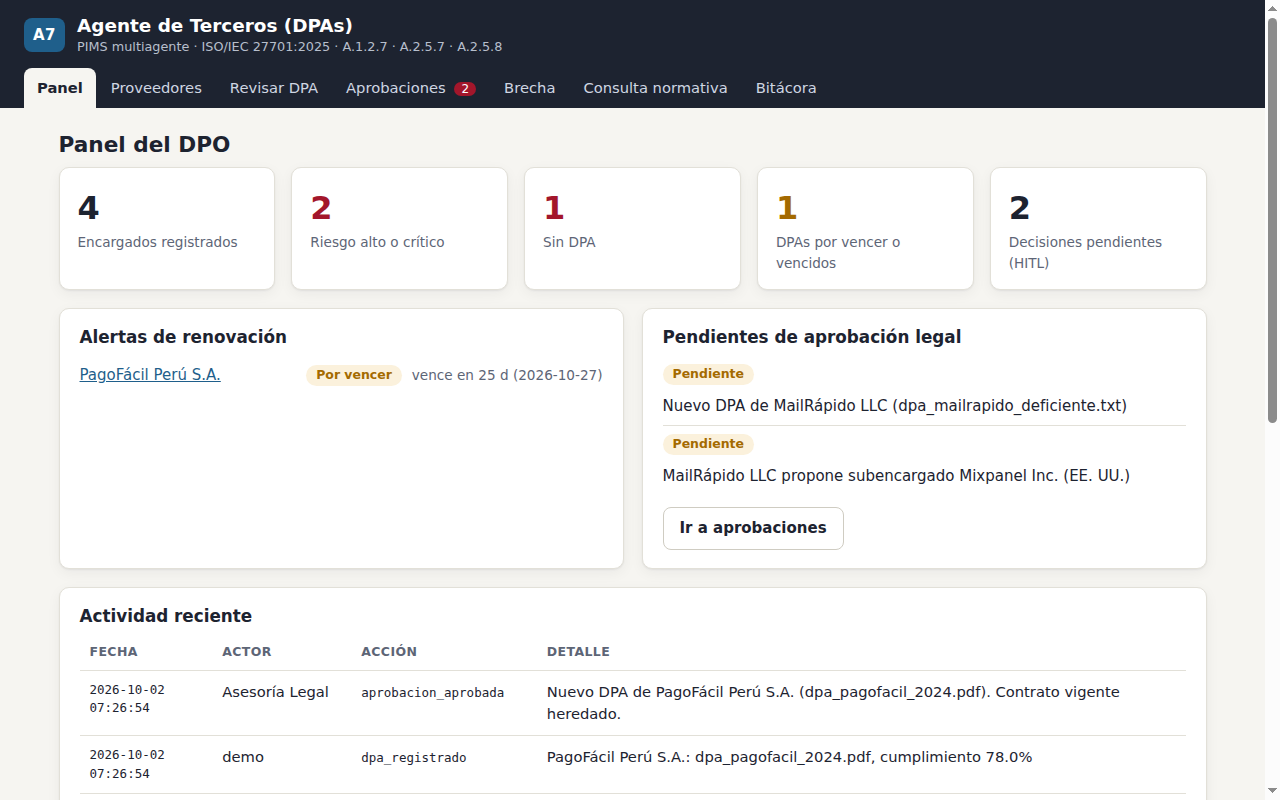
\includegraphics[width=\linewidth]{../figuras/panel.png}
\column{.5\textwidth}
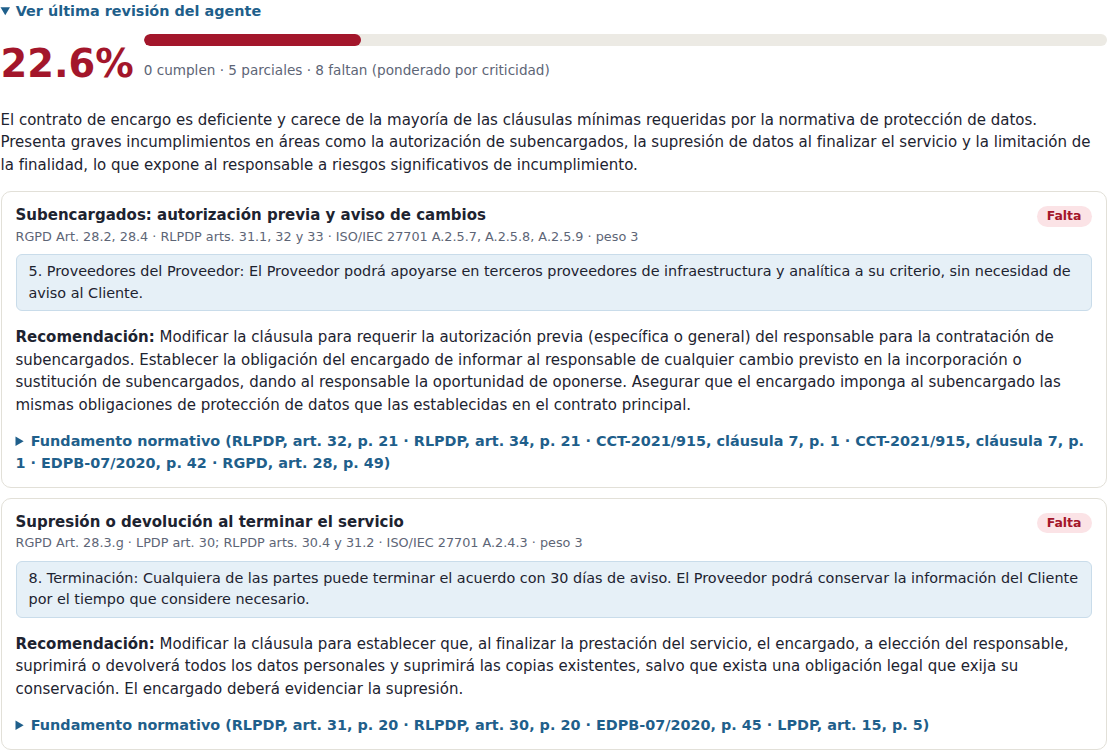
\includegraphics[width=\linewidth]{../figuras/revision.png}
\end{columns}
\vspace{4pt}
\small Panel del DPO (alertas y decisiones pendientes) e informe de revisión con citas literales y fundamentos (fuente, artículo, página).
\end{frame}

\begin{frame}{Riesgo, subencargados y brechas}
\begin{columns}[c]
\column{.5\textwidth}
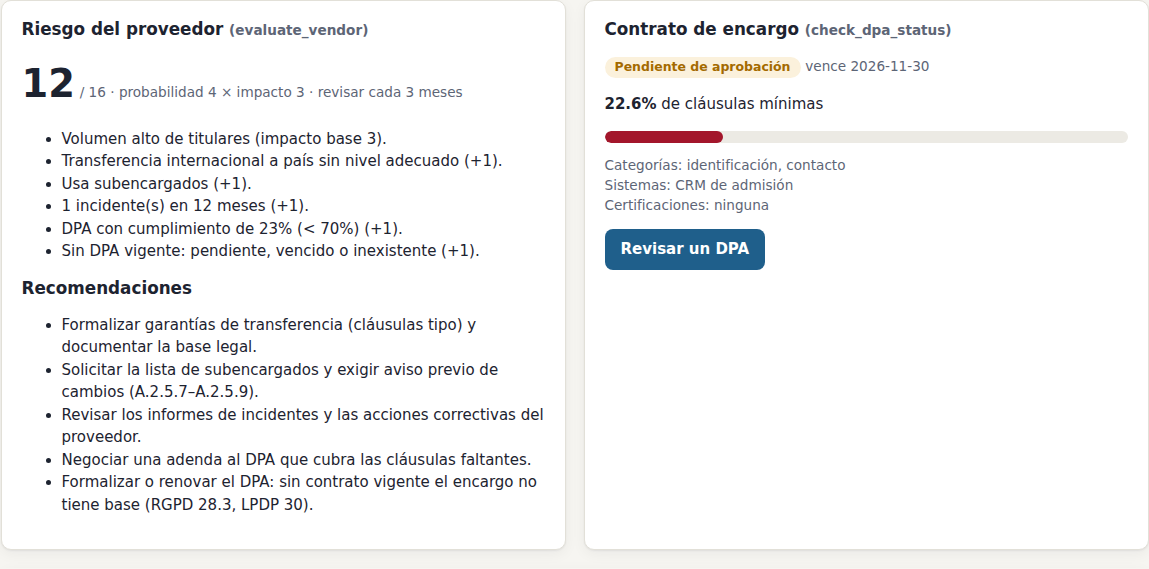
\includegraphics[width=\linewidth]{../figuras/riesgo.png}
\column{.5\textwidth}
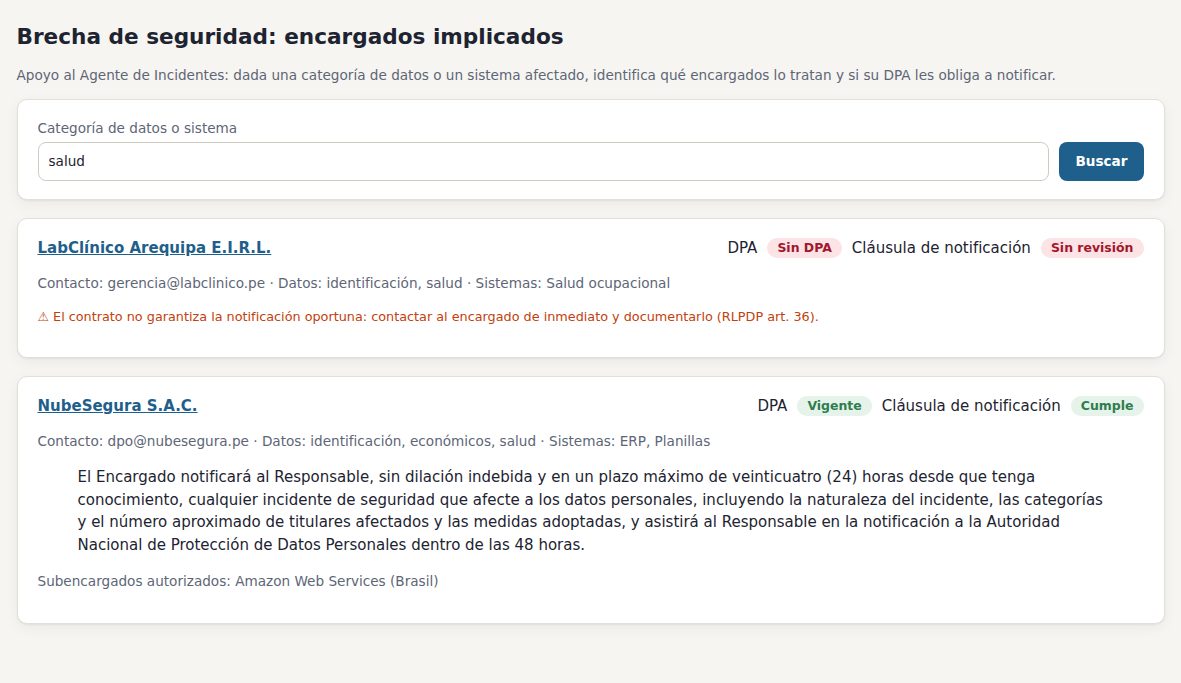
\includegraphics[width=\linewidth]{../figuras/brecha.png}
\end{columns}
\vspace{4pt}
\small Ficha del proveedor (\texttt{evaluate\_vendor}, \texttt{check\_dpa\_status}) y encargados implicados en una brecha de datos de salud.
\end{frame}

\begin{frame}{Limitaciones y trabajo futuro}
\begin{columns}[T]
\column{.5\textwidth}
\textbf{Limitaciones}
\begin{itemize}\small
  \item Evaluación pequeña (3 contratos, anotados por los autores).
  \item El LLM no es determinista $\rightarrow$ verificación literal + HITL.
  \item ISO/IEC 27701:2025 no es de libre acceso: numeración inferida.
  \item Falta OCR para PDFs escaneados.
\end{itemize}
\column{.5\textwidth}
\textbf{Trabajo futuro}
\begin{itemize}\small
  \item Integración con el orquestador y los agentes de Incidentes y Controles por MCP.
  \item Migración a la base PostgreSQL central del PIMS.
  \item Generación de adendas contractuales.
  \item Contratos reales anonimizados, anotados con un abogado.
\end{itemize}
\end{columns}
\end{frame}

\begin{frame}[standout]
¡Gracias!\\[6pt]
\normalsize github.com/S-kkipie/agente-terceros-dpa
\end{frame}

\end{document}
